
%%
%% Lab 7 report content. Retain the document preamble and package definitions
%% used for the previous laboratory reports.
\title{LAB 7: Plate Bending, Shear Locking, and Hourglassing}

\author{Adhilsha A (SE25PCSE007)}
\maketitle

\tableofcontents

\section{Introduction}

This laboratory investigates the bending response of shell and solid finite
elements. The first problem studies the mesh convergence and thickness
dependence of a clamped square plate subjected to uniform transverse pressure.
The second problem compares different solid-element formulations for a
clamped steel strip subjected to a transverse tip load. The results
demonstrate mesh convergence, bending stress reversal through the thickness,
transverse-shear effects in thick plates, shear locking, reduced-integration
hourglassing, and the advantages of enhanced-strain and higher-order
elements.

All calculations use mm, N, and MPa. The material properties are
\[
E=\SI{200000}{\mega\pascal},\qquad \nu=0.3.
\]

\section{Problem 1: Clamped Square Plate}

\subsection{Geometry, Material, and Loading}

The plate is a \(\SI{1000}{\milli\metre}\times\SI{1000}{\milli\metre}\)
square modelled using \texttt{SHELL181}. A uniform transverse pressure
\(q=\SI{0.01}{\mega\pascal}\) is applied over the plate, and all four edges
are clamped. The plate thickness for the mesh-convergence and stress studies
is \(t=\SI{10}{\milli\metre}\).

\begin{table}[h!]
\centering
\begin{tabular}{ll}
\toprule
\textbf{Quantity} & \textbf{Value} \\
\midrule
Plate dimensions & $1000\ \mathrm{mm}\times1000\ \mathrm{mm}$ \\
Thickness for parts (a) and (b) & $10\ \mathrm{mm}$ \\
Young's modulus & $200000\ \mathrm{MPa}$ \\
Poisson's ratio & $0.30$ \\
Uniform pressure & $0.01\ \mathrm{MPa}$ \\
Boundary condition & All four edges clamped \\
Element & SHELL181 \\
\bottomrule
\end{tabular}
\caption{Problem 1 input data}
\end{table}

\subsection{APDL Code}

The mesh-convergence, surface-stress, and thickness-variation calculations
were performed using the following APDL input:

\lstinputlisting[style=pyconsole]{codes/lab7_1.txt}

\subsection{Mesh Convergence}

The centre deflection \(U_Z\) was extracted at
\((x,y)=(500,500)\) mm for \(4\times4\), \(8\times8\), and \(20\times20\)
meshes. The three meshes are shown in
Figures~\ref{lab7_mesh_4}--\ref{lab7_mesh_20}. The \(U_Z\) contours are
shown in Figures~\ref{lab7_uz_4}--\ref{lab7_uz_20}.

\begin{figure}[!h]
\centering
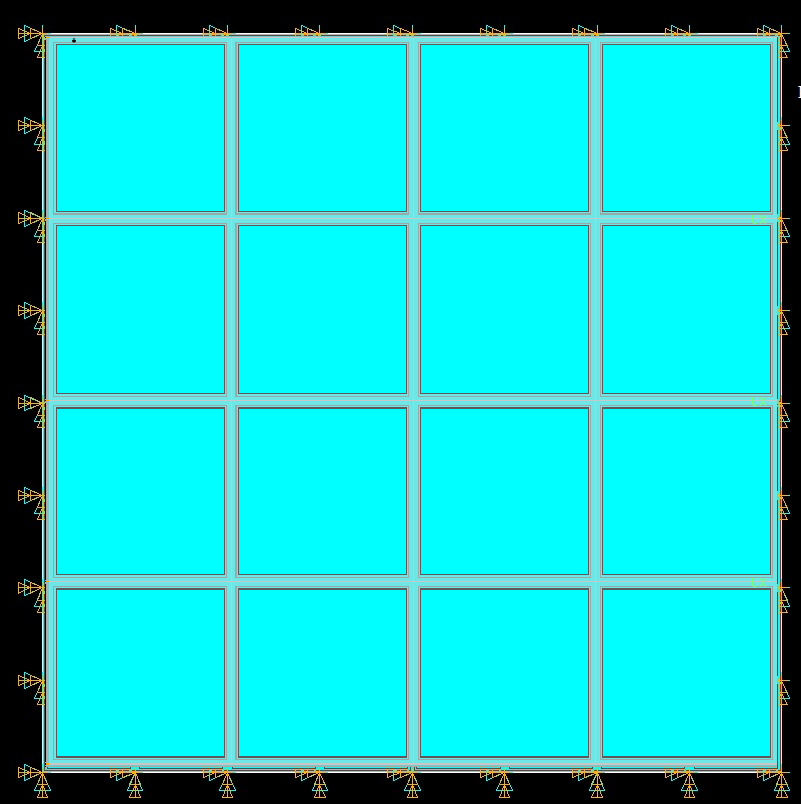
\includegraphics[width=0.5\linewidth]{figures/lab7_1_mesh_4x4.png}
\caption{$4\times4$ mesh used in the convergence study}
\label{lab7_mesh_4}
\end{figure}

\begin{figure}[!h]
\centering
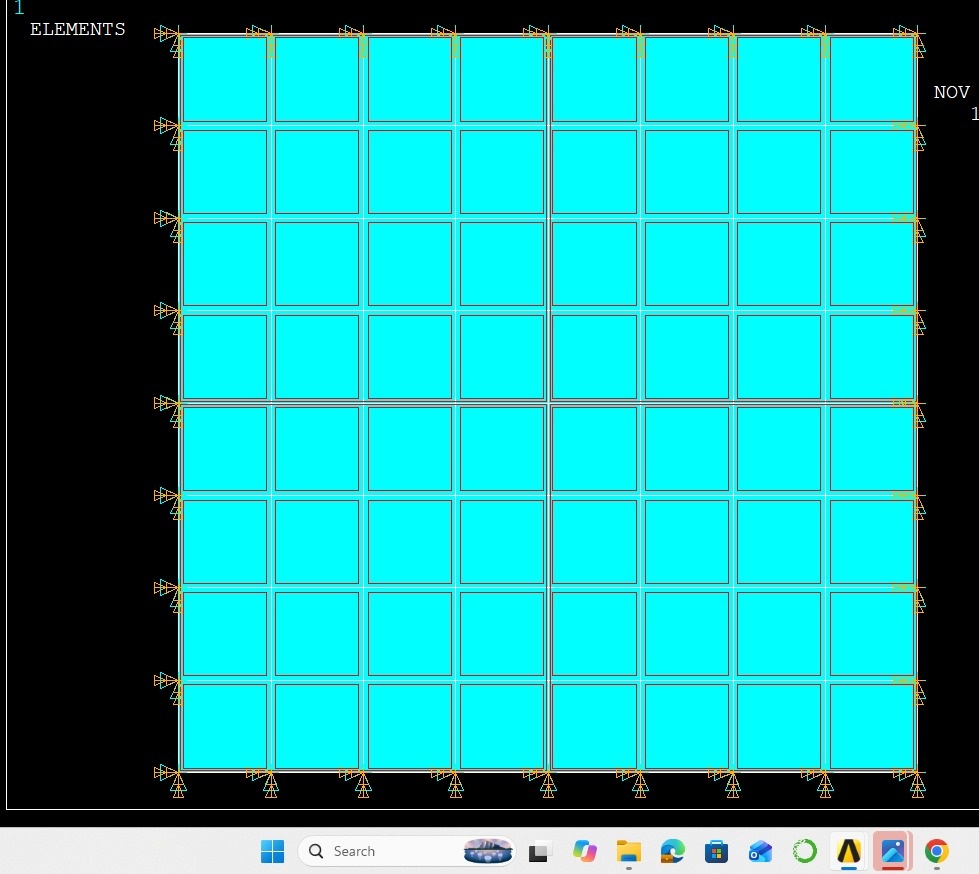
\includegraphics[width=0.5\linewidth]{figures/lab7_1_mesh_8x8.jpeg}
\caption{$8\times8$ mesh used in the convergence study}
\label{lab7_mesh_8}
\end{figure}

\begin{figure}[!h]
\centering
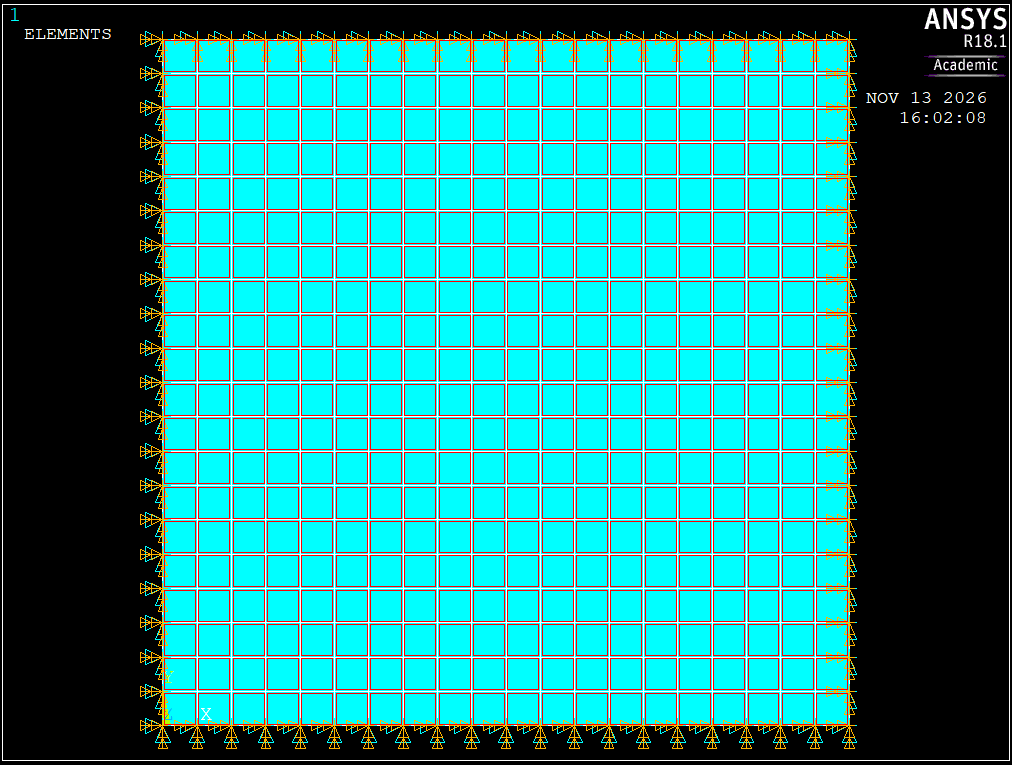
\includegraphics[width=0.5\linewidth]{figures/lab7_1_0.png}
\caption{$20\times20$ mesh used in the convergence study}
\label{lab7_mesh_20}
\end{figure}

\begin{figure}[!h]
\centering
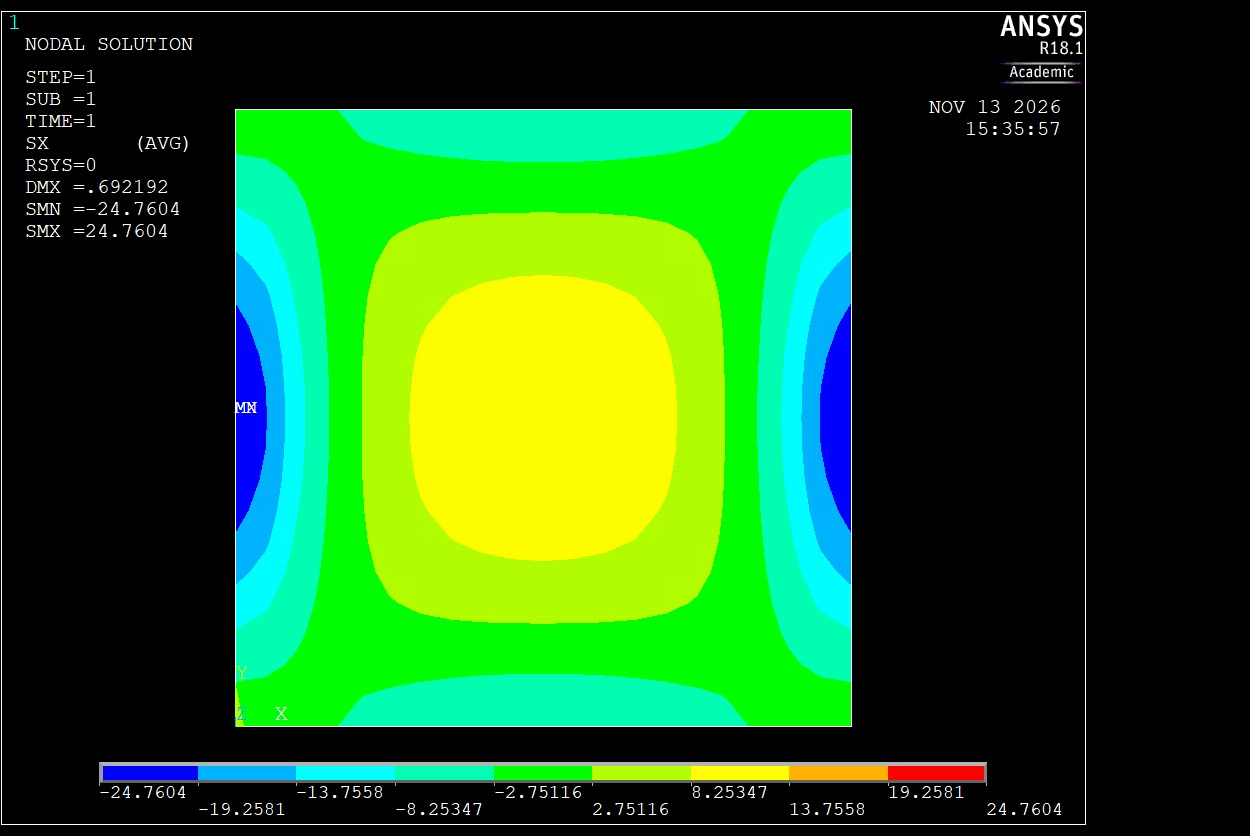
\includegraphics[width=0.70\linewidth]{figures/lab7_1_Uz_4x4.jpeg}
\caption{Centre deflection contour for the $4\times4$ mesh}
\label{lab7_uz_4}
\end{figure}

\begin{figure}[!h]
\centering
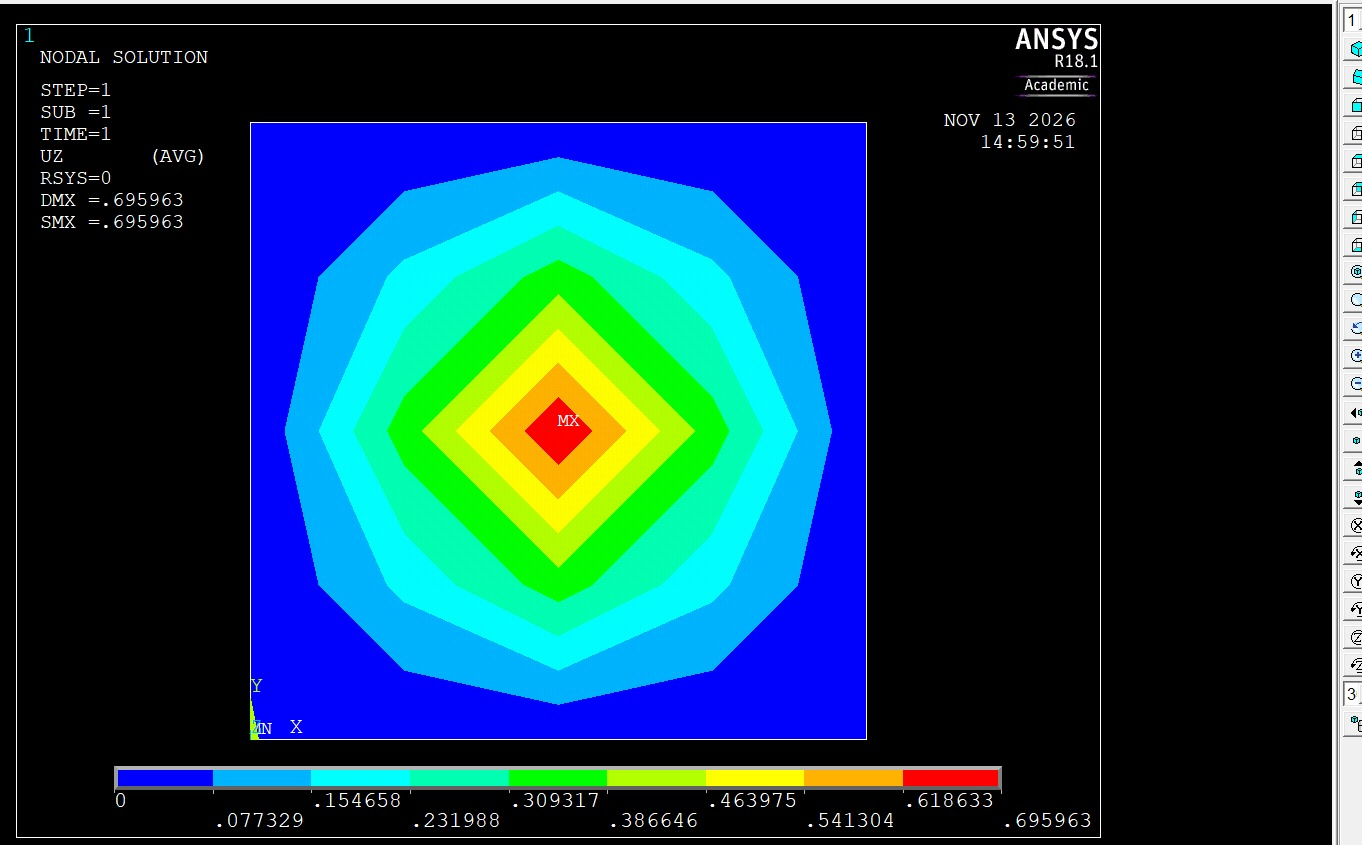
\includegraphics[width=0.70\linewidth]{figures/lab7_1_Uz_8x8.jpeg}
\caption{Centre deflection contour for the $8\times8$ mesh}
\label{lab7_uz_8}
\end{figure}

\begin{figure}[!h]
\centering
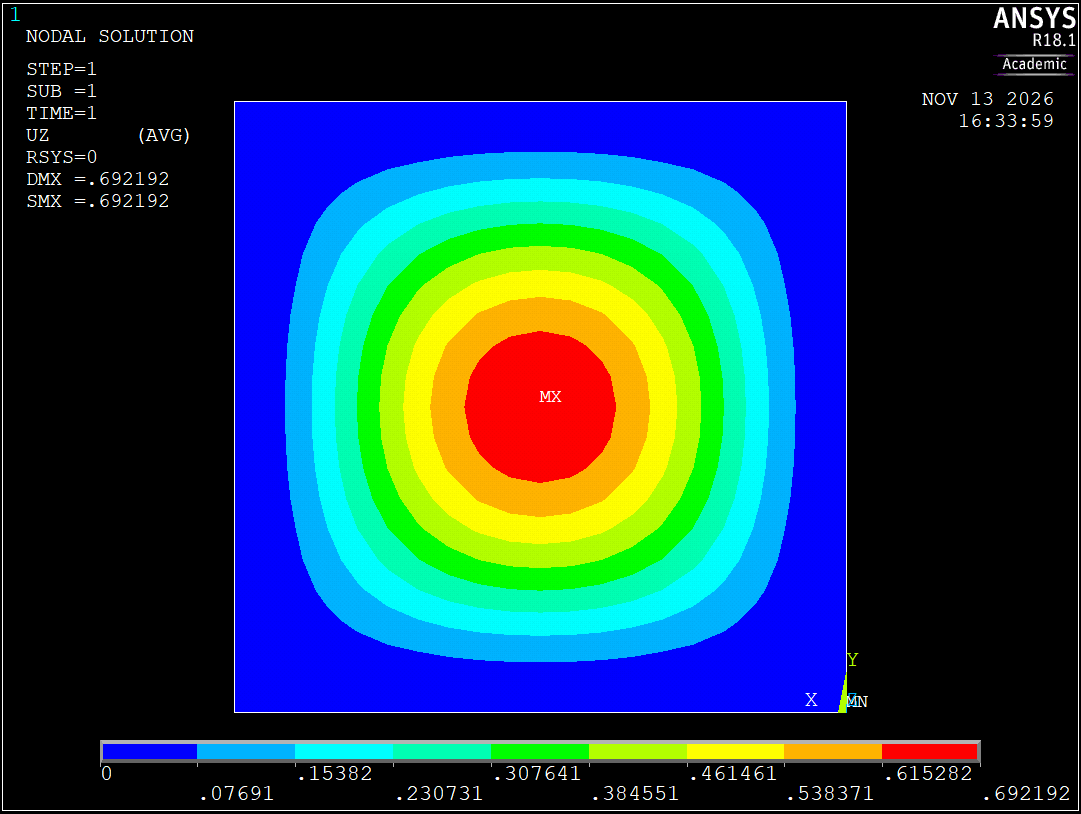
\includegraphics[width=0.70\linewidth]{figures/lab7_1_5_Uz.png}
\caption{Centre deflection contour for the $20\times20$ mesh}
\label{lab7_uz_20}
\end{figure}

The extracted centre deflections are:

\begin{table}[h!]
\centering
\begin{tabular}{c|c|c|c|c}
\toprule
\textbf{Mesh} & \textbf{Element size (mm)} &
\textbf{Centre }U_Z\textbf{ (mm)} &
\textbf{Kirchhoff }w\textbf{ (mm)} & \textbf{FE/reference}\\
\midrule
$4\times4$ & 250 & $-0.695926604$ & $-0.687960$ & $1.0116$\\
$8\times8$ & 125 & $-0.692108687$ & $-0.687960$ & $1.0060$\\
$20\times20$ & 50 & $-0.692191830$ & $-0.687960$ & $1.0062$\\
\bottomrule
\end{tabular}
\caption{Mesh-convergence results for the plate centre}
\label{tab:plate-convergence}
\end{table}

For \(t=\SI{10}{\milli\metre}\),
\[
D=\frac{Et^3}{12(1-\nu^2)}
=\SI{18315018.32}{\newton\milli\metre},
\qquad
w_{\mathrm K}=0.00126\frac{qa^4}{D}
=\SI{0.68796}{\milli\metre}.
\]
The displacement changes very little after refining the mesh from
\(8\times8\) to \(20\times20\). Thus, the \(20\times20\) result is taken as
the converged finite-element value,
\[
|U_Z|_{\mathrm{converged}}\approx\SI{0.69219}{\milli\metre}.
\]
The smooth, concentric contours in the displacement plots also indicate that
the response is symmetric about the centre of the plate.

\subsection{Top and Bottom Surface Stresses}

For the converged \(20\times20\) mesh, the \(x\)-normal stress was plotted on
the top and bottom shell surfaces. The results are shown in
Figures~\ref{lab7_stress_top} and \ref{lab7_stress_bottom}.

\begin{figure}[!h]
\centering
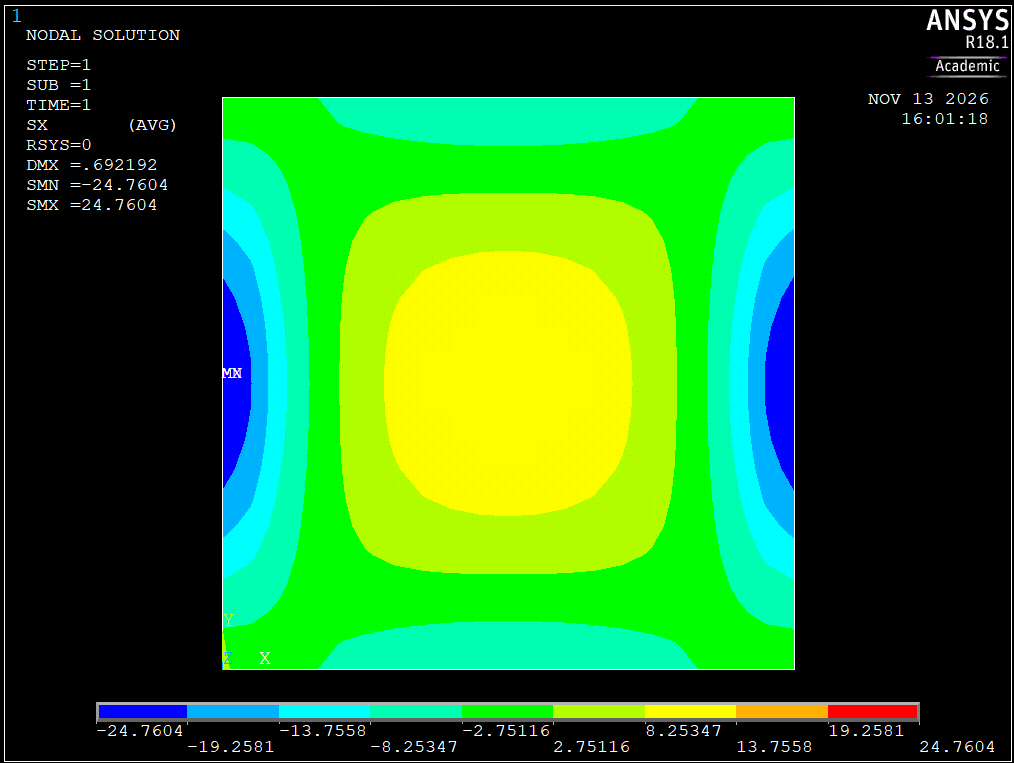
\includegraphics[width=0.72\linewidth]{figures/lab7_1_1_sigmax_top.png}
\caption{Top-surface \(\sigma_x\) contour for the \(\SI{10}{\milli\metre}\) plate}
\label{lab7_stress_top}
\end{figure}

\begin{figure}[!h]
\centering
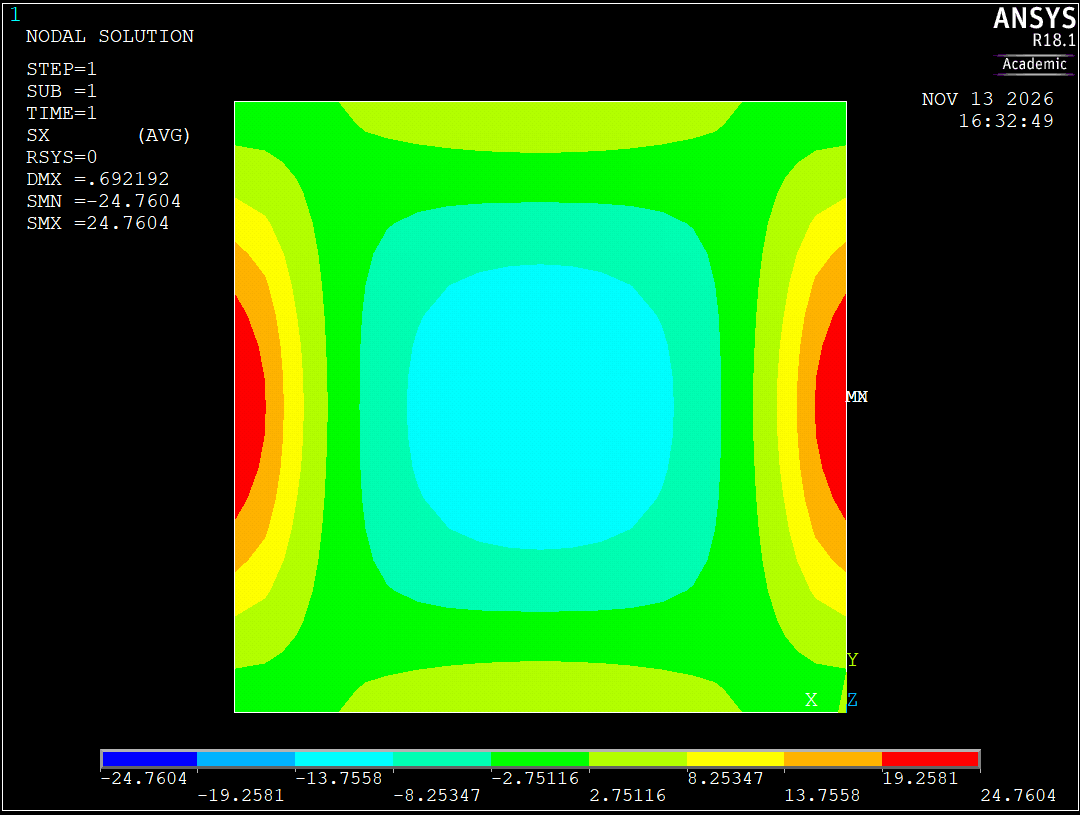
\includegraphics[width=0.72\linewidth]{figures/lab7_1_2_sigmax_bottom.png}
\caption{Bottom-surface \(\sigma_x\) contour for the \(\SI{10}{\milli\metre}\) plate}
\label{lab7_stress_bottom}
\end{figure}

The stress range on the top surface is approximately
\[
-\SI{24.7604}{\mega\pascal}\leq\sigma_x
\leq\SI{24.7604}{\mega\pascal},
\]
and the bottom surface has the same magnitude with the opposite bending
sign. The top and bottom stresses are equal and opposite because bending
stress varies linearly through the thickness:
\[
\sigma_x(z)=\frac{M_xz}{I}.
\]
The neutral surface has \(z=0\), while the top and bottom surfaces are at
\(z=\pm t/2\). The stress therefore reverses sign between the two faces.
The largest bending stress occurs near the restrained edges, where the
clamped boundary develops the largest bending moments. The stress contours
are symmetric because both the geometry and the pressure loading are
symmetric.

The reference edge moment given in the question is
\[
M=0.0513qa^2
 =0.0513(0.01)(1000)^2
 =\SI{513}{\newton\milli\metre\per\milli\metre}.
\]
Therefore, the reference outer-fibre stress is
\[
\sigma_{\mathrm{ref}}=\frac{6M}{t^2}
=\frac{6(513)}{10^2}
=\SI{30.78}{\mega\pascal}.
\]
The finite-element peak value of \(\SI{24.7604}{\mega\pascal}\) is
approximately \(19.6\%\) lower than this reference estimate. The difference
is attributable to the analytical moment coefficient versus the interpolated
nodal shell stress and the finite mesh. The opposite signs on the two
surfaces are required by the change from \(z=+t/2\) to \(z=-t/2\).

\subsection{Thickness Variation}

The \(20\times20\) mesh was retained while the shell thickness was changed.
The corresponding aspect ratios and centre deflections are:

\begin{table}[h!]
\centering
\begin{tabular}{c|c|c|c|c}
\toprule
\textbf{Thickness (mm)} & \textbf{$a/t$} &
\textbf{FE centre }U_Z\textbf{ (mm)} &
\textbf{Kirchhoff estimate (mm)} & \textbf{FE/Kirchhoff}\\
\midrule
10  & 100 & $-0.692191830$ & $-0.687960$ & $1.006$\\
50  & 20  & $-0.0057956$ & $-0.005504$ & $1.053$\\
100 & 10  & $-0.0008212$ & $-0.0006879$ & $1.194$\\
200 & 5   & $-0.0001482$ & $-0.0000860$ & $1.724$\\
\bottomrule
\end{tabular}
\caption{Centre deflection as a function of shell thickness}
\label{tab:thickness}
\end{table}

For the thin plate, the classical Kirchhoff bending result is used as the
reference. Since the bending rigidity varies as \(D\propto t^3\), the
Kirchhoff deflection varies approximately as
\[
w_{\mathrm{K}}(t)=w_{\mathrm{K}}(10)
\left(\frac{10}{t}\right)^3.
\]
The finite-element values become increasingly larger than the Kirchhoff
values as the plate becomes thicker. This is expected because
\texttt{SHELL181} is based on Mindlin--Reissner shell theory and includes
transverse shear deformation. Kirchhoff theory neglects transverse shear,
so its error increases as \(a/t\) decreases. The thickness-study parameter
listing and stress result are shown in Figure~\ref{lab7_thickness_status}.

\begin{figure}[!h]
\centering
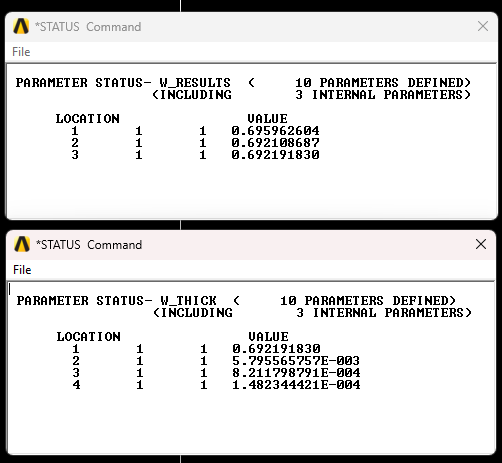
\includegraphics[width=0.72\linewidth]{figures/lab7_1_4.png}
\caption{APDL parameter listing for the thickness study}
\label{lab7_thickness_status}
\end{figure}

The complete convergence and thickness parameter output is also shown in
Figure~\ref{lab7_parameter_output}.  It confirms the values tabulated above
and shows that the mesh-convergence values and the thickness-study values
were generated from separate result arrays.

\begin{figure}[!h]
\centering
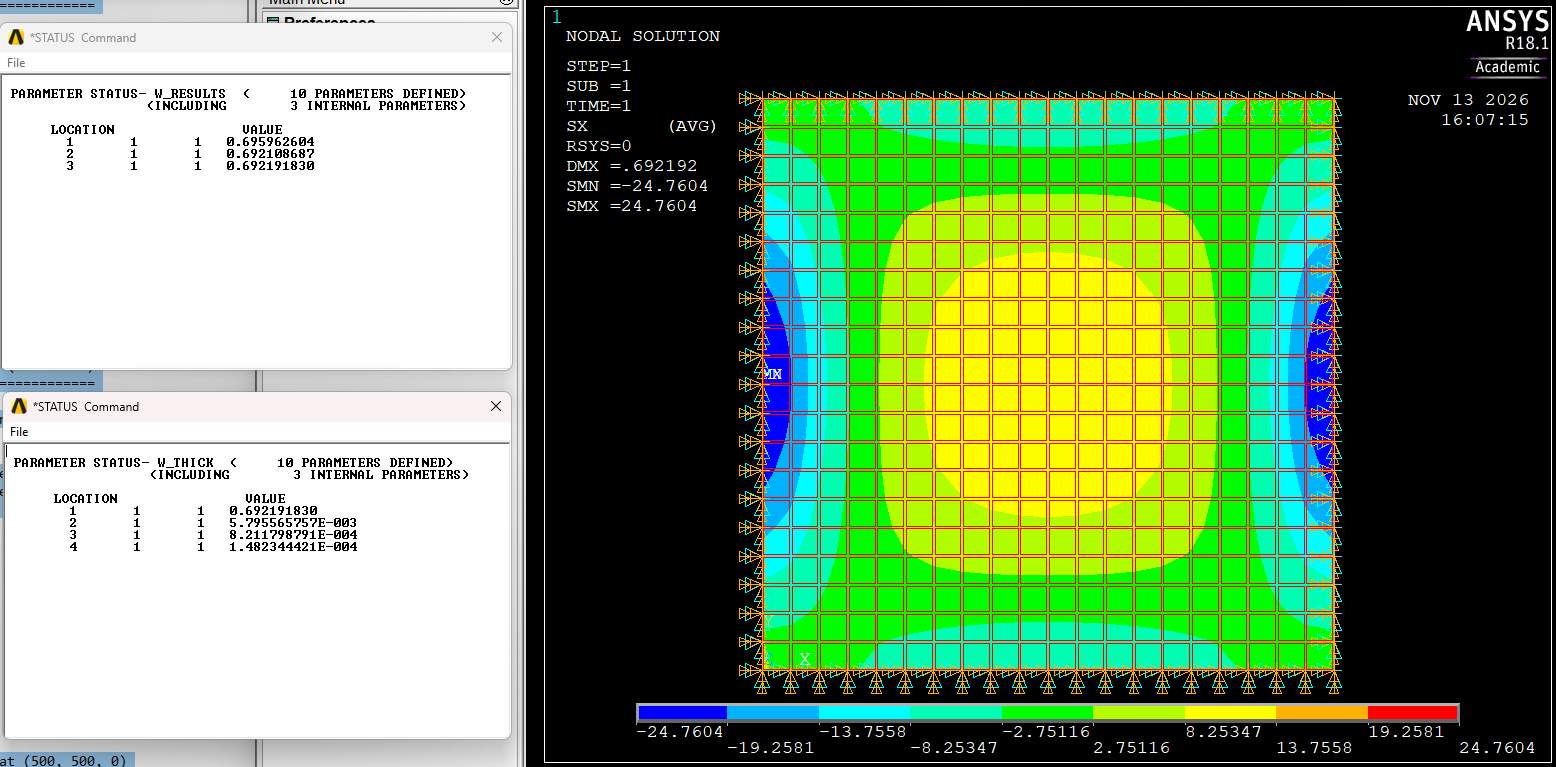
\includegraphics[width=0.78\linewidth]{figures/lab7_1_3.png}
\caption{APDL parameter output and the converged stress contour}
\label{lab7_parameter_output}
\end{figure}

\section{Problem 2: Solid-Element Bending of a Steel Strip}

\subsection{Geometry and Analytical Reference}

The second problem considers a clamped steel strip of length
\(L=\SI{200}{\milli\metre}\), width \(b=\SI{20}{\milli\metre}\), and thickness
\(t=\SI{5}{\milli\metre}\). A transverse tip load
\(P=\SI{10}{\newton}\) is applied at \(x=L\). The solid strip has a
\(20\times2\times1\) mesh for the \(x\), \(y\), and \(z\) directions.

\begin{table}[h!]
\centering
\begin{tabular}{ll}
\toprule
\textbf{Quantity} & \textbf{Value}\\
\midrule
Length, $L$ & $200\ \mathrm{mm}$\\
Width, $b$ & $20\ \mathrm{mm}$\\
Thickness, $t$ & $5\ \mathrm{mm}$\\
Tip load, $P$ & $10\ \mathrm{N}$ downward\\
Second moment, $I=bt^3/12$ & $208.333\ \mathrm{mm}^4$\\
\bottomrule
\end{tabular}
\caption{Problem 2 input data}
\end{table}

The Euler--Bernoulli reference displacement is
\[
I=\frac{bt^3}{12}
=\frac{20(5)^3}{12}
=\SI{208.333}{\milli\metre^4},
\]
\[
\delta_{\mathrm{EB}}=\frac{PL^3}{3EI}
=-\frac{10(200)^3}{3(200000)(208.333)}
=-\SI{0.64}{\milli\metre}.
\]
The displacement is negative because the applied load acts in the negative
\(z\)-direction.

\subsection{APDL Code}

The full-integration, reduced-integration, enhanced-strain, SOLID186, and
SHELL181 analyses were performed using:

\lstinputlisting[style=pyconsole]{codes/lab7_2.txt}

\subsection{Full Integration Results}

An example result from ANSYS for \(20\times2\times1\) SOLID185 full
integration is given in Figure~\ref{lab7_full_sample}. The fully integrated
\texttt{SOLID185} model with different mesh sizes gave the tip deflections
summarized in Table~\ref{tab:full-integration}.

\begin{figure}[!h]
\centering
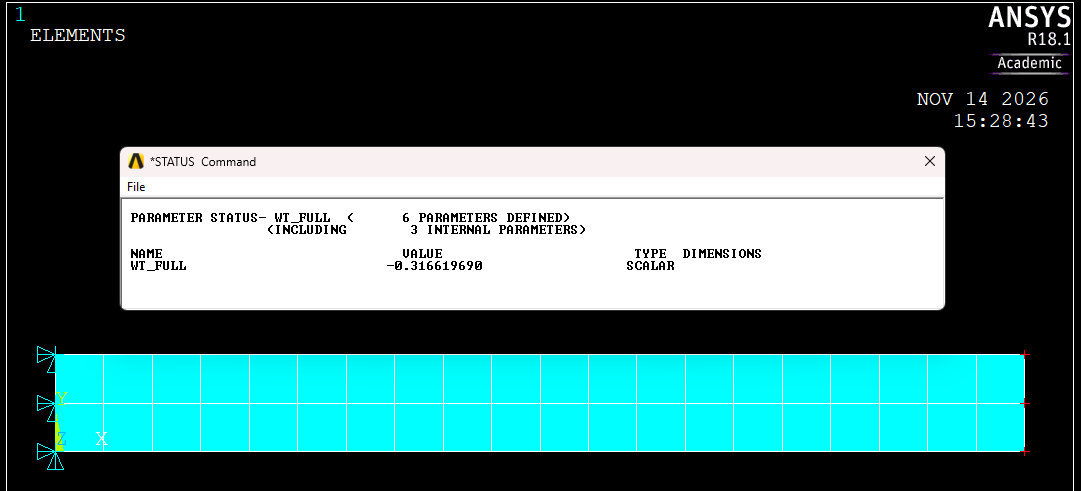
\includegraphics[width=0.72\linewidth]{figures/lab7_2_a_new.png}
\caption{Full-integration SOLID185 result for the $20\times2\times1$ mesh}
\label{lab7_full_sample}
\end{figure}

\begin{table}[h!]
\centering
\caption{Full-integration SOLID185 mesh refinement results}
\label{tab:full-integration}
\renewcommand{\arraystretch}{1.3}
\begin{tabular}{|c|c|c|c|}
\hline
\textbf{Mesh Configuration} & \textbf{FEA Deflection} & \textbf{Beam Deflection} & \textbf{Ratio} \\
$(L \times W \times t)$ & $\delta_{\text{FE}}$ (mm) & $\delta_{\text{beam}}$ (mm) & $\delta_{\text{FE}} / \delta_{\text{beam}}$ \\
\hline
$20 \times 2 \times 1$ & $-0.317$ & $-0.64$ & $0.495$ \\
\hline
$20 \times 2 \times 2$ & $-0.257$ & $-0.64$ & $0.401$ \\
\hline
$20 \times 2 \times 4$ & $-0.248$ & $-0.64$ & $0.387$ \\
\hline
$80 \times 2 \times 1$ & $-1.106$ & $-0.64$ & $1.728$ \\
\hline
\end{tabular}
\end{table}

The tip deflection from $20\times2\times1$ is smaller in magnitude than the Euler--Bernoulli value because the
first-order fully integrated brick is excessively stiff in this
bending-dominated, thin-strip mesh. The result is a typical manifestation of
shear locking: the element cannot represent the nearly pure bending field
without introducing spurious transverse shear strains. Linear interpolation functions restrict the ability of the elements to represent the curvature associated with bending deformation.

Adding elements through the thickness moves the result from
\(-0.317\) mm to \(-0.257\) mm and then \(-0.248\) mm. It therefore changes
the response, but these values remain smaller in magnitude than the beam
reference and do not by themselves establish convergence. Through-thickness
refinement helps because it reduces the element's constrained bending
deformation and improves representation of the strain variation from the
top to the bottom surface.

The \(80\times2\times1\) longitudinal refinement produces
\(-1.106\) mm, giving a ratio of \(1.728\) relative to the beam reference.
This refinement is separate from the through-thickness refinements and
therefore is not required to follow the preceding thickness-refinement
trend. Its increased flexibility with longitudinal refinement is consistent
with the change in element aspect ratio and reduced bending stiffness,
although the value should be interpreted as the result of this specific
finite-element mesh rather than as a monotonic continuation of the
through-thickness sequence.

\subsection{Reduced Integration results}

For the reduced-integration model, the distributed tip load is first solved
and then a second solution is performed with the load concentrated at a
single corner node. The latter is intended to expose hourglass deformation.
The resulting scaled displacement plot is shown in
Figure~\ref{lab7_hourglass}. The displayed value is approximately
\(-\SI{110.885}{\milli\metre}\), which is not a converged physical beam
deflection. It is an unstable zero-energy mode caused by insufficient
integration constraints. Reduced integration removes locking but introduces
hourglass modes; hourglass control limits these modes but does not make an
arbitrarily concentrated load a reliable bending test. The correct ratio for
this single-node demonstration is
\[
\frac{\delta_{\mathrm{FE}}}{\delta_{\mathrm{beam}}}
=\frac{-110.885}{-0.64}=173.26,
\]
not a physical deflection ratio. It is reported only to demonstrate the
hourglass mechanism.

We further repeat the same setting with 4 element thickness and the result is added in Figure~\ref{lab7_hourglass_thick4} where the value is approximately
\(-\SI{0.677}{\milli\metre}\). Compared to the analytical value of 0.64, the deflection ratio $\delta_{FE} / \delta_{beam} = 1.06$, which is much better compared to thickness with 1 element. This shows that reduced integration can give us accurate bending result given an appropriate mesh. It is to be noted that an inappropriate meshing or thickness discretization can introduce hourglasses. 

\begin{figure}[!h]
\centering
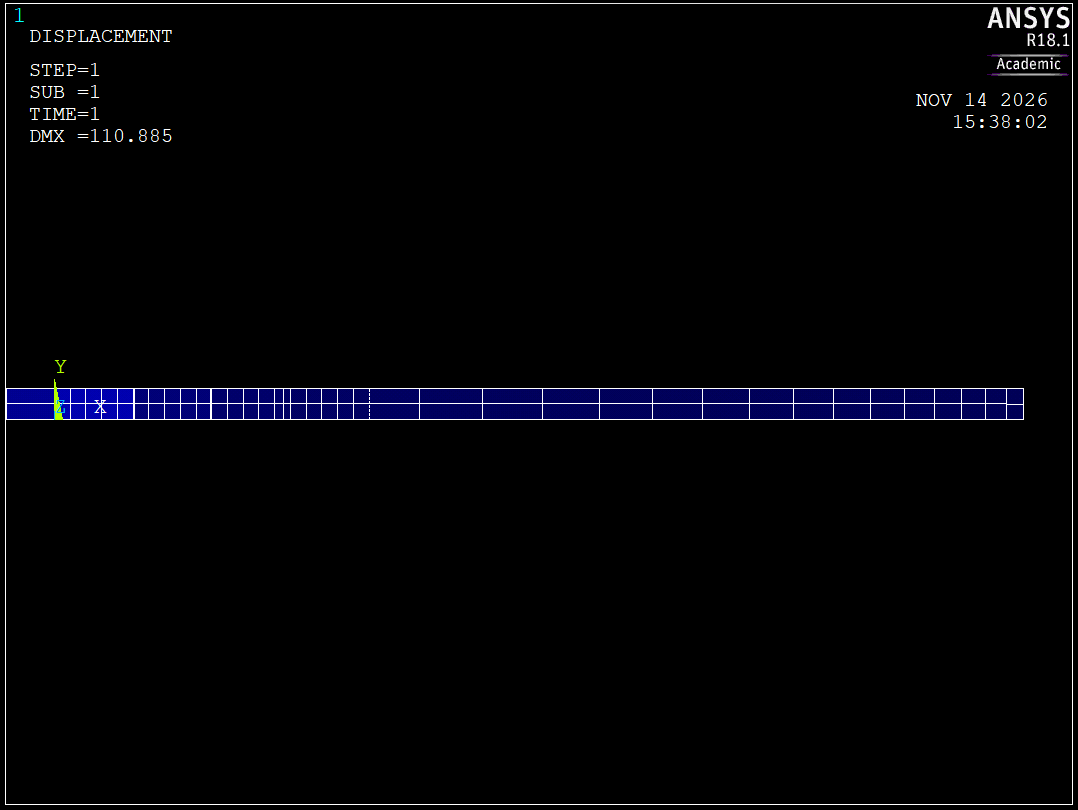
\includegraphics[width=0.72\linewidth]{figures/lab7_2_b_displacement_new.png}
\caption{Scaled reduced-integration response during the single-node hourglass test}
\label{lab7_hourglass}
\end{figure}
\begin{figure}[!h]
\centering
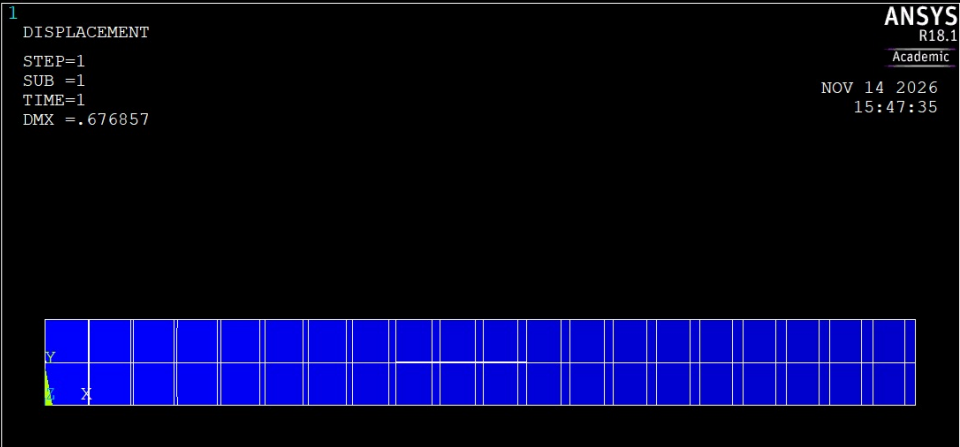
\includegraphics[width=0.72\linewidth]{figures/lab7_2_b_displacement_thick4.png}
\caption{Scaled reduced-integration response with 4 element thickness}
\label{lab7_hourglass_thick4}
\end{figure}

\subsection{Comparison of Element Formulations}

The enhanced-strain \texttt{SOLID185}, twenty-node \texttt{SOLID186}, and
\texttt{SHELL181} results are shown in Figures~\ref{lab7_enhanced}-\ref{lab7_shell}.
The extracted tip values are given in Table~\ref{tab1} below:

\begin{table}[h!]
\centering
\caption{Better element results}
\label{tab1}
\renewcommand{\arraystretch}{1.3} % Adds vertical padding for readability
\begin{tabular}{|c|c|c|c|}
\hline
\textbf{Mesh and Element Configuration} & \textbf{FEA Deflection} & \textbf{Beam Deflection} & \textbf{Ratio} \\
 & $\delta_{\text{FE}}$ (mm) & $\delta_{\text{beam}}$ (mm) & $\delta_{\text{FE}} / \delta_{\text{beam}}$ \\
\hline
$20 \times 2 \times 1$ SOLID185 & $-0.634$ & $-0.64$ & $0.991$ \\
\hline
$20 \times 2 \times 1$ SOLID186 & $-0.631$ & $-0.64$ & $0.986$ \\
\hline
$20 \times 2$ SHELL181 & $-0.635$ & $-0.64$ & $0.992$ \\
\hline
\end{tabular}
\end{table}

All of the above advanced elements provide deflections close to the
analytical value of −0.64 mm. Their accuracy shows us the importance of selecting suitable elements according to the problem so as to effectively reduce shear locking and improve numerical performance without extensive mesh refinement.

\subsection{Complete comparison}

\begin{table}[h!]
\centering
\begin{tabular}{|l|c|c|c|}
\toprule
\textbf{Formulation / mesh} & \textbf{Tip }U_Z\textbf{ (mm)}
& $\delta_{\mathrm{FE}}/\delta_{\mathrm{beam}}$ & \textbf{Observation}\\
\midrule
$20\times2\times1$ SOLID185, full & $-0.316620$ & $0.495$ & Shear locking\\
$20\times2\times2$ SOLID185, full & $-0.257$ & $0.402$ & Stiffer than the beam reference\\
$20\times2\times4$ SOLID185, full & $-0.248$ & $0.388$ & Through-thickness refinement\\
$80\times2\times1$ SOLID185, full & $-1.106$ & $1.728$ & Longitudinal refinement result\\
$20\times2\times1$ SOLID185, reduced, single-node & $-110.885$ & $173.26$ & Hourglass demonstration, not physical\\
$20\times2\times4$ SOLID185, reduced & $-0.677$ & $1.058$ & Improved with thickness refinement\\
$20\times2\times1$ SOLID185, enhanced strain & $-0.634$ & $0.991$ & Close to beam reference\\
$20\times2\times1$ SOLID186 & $-0.631$ & $0.986$ & Higher-order brick\\
$20\times2$ SHELL181 & $-0.635$ & $0.992$ & Mid-surface shell model\\
Euler--Bernoulli reference & $-0.640$ & $1.000$ & Reference value\\
\bottomrule
\end{tabular}
\caption{Complete displacement comparison for Problem 2}
\label{tab:solid-comparison}
\end{table}

\begin{figure}[!h]
\centering
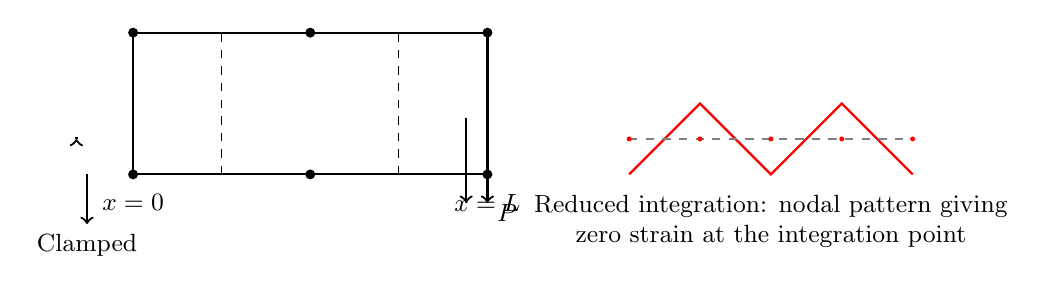
\begin{tikzpicture}[scale=0.9, every node/.style={font=\small}]
    % Rectangular 8-node brick
    \draw[thick] (0,0) rectangle (5,2);
    \draw[dashed] (1.25,0) -- (1.25,2);
    \draw[dashed] (3.75,0) -- (3.75,2);
    \node[below] at (0,-0.15) {$x=0$};
    \node[below] at (5,-0.15) {$x=L$};
    \foreach \x in {0,2.5,5}{
        \fill (\x,0) circle (2pt);
        \fill (\x,2) circle (2pt);
    }
    \draw[->,thick] (-0.8,0.5) -- (-0.8,0.5) node[left] {};
    \draw[thick,->] (-0.65,0) -- (-0.65,-0.7) node[below] {Clamped};
    \draw[thick,->] (5,0.8) -- (5,-0.4);
    \draw[thick,->] (4.7,0.8) -- (4.7,-0.4);
    \node[right] at (5,-0.55) {$P$};

    % Distorted hourglass shape
    \draw[thick,red] (7,0) -- (8.0,1.0) -- (9.0,0)
                    -- (10,1.0) -- (11,0);
    \draw[dashed,gray] (7,0.5) -- (11,0.5);
    \foreach \x in {7,8,9,10,11}{
        \fill[red] (\x,0.5) circle (1pt);
    }
    \node[align=center,below] at (9,-0.15)
        {Reduced integration: nodal pattern giving\\
        zero strain at the integration point};
\end{tikzpicture}
\caption{Sketch of an 8-node brick in a bending strip and a characteristic reduced-integration hourglass pattern}
\label{lab7_element_sketch}
\end{figure}

\begin{figure}[!h]
\centering
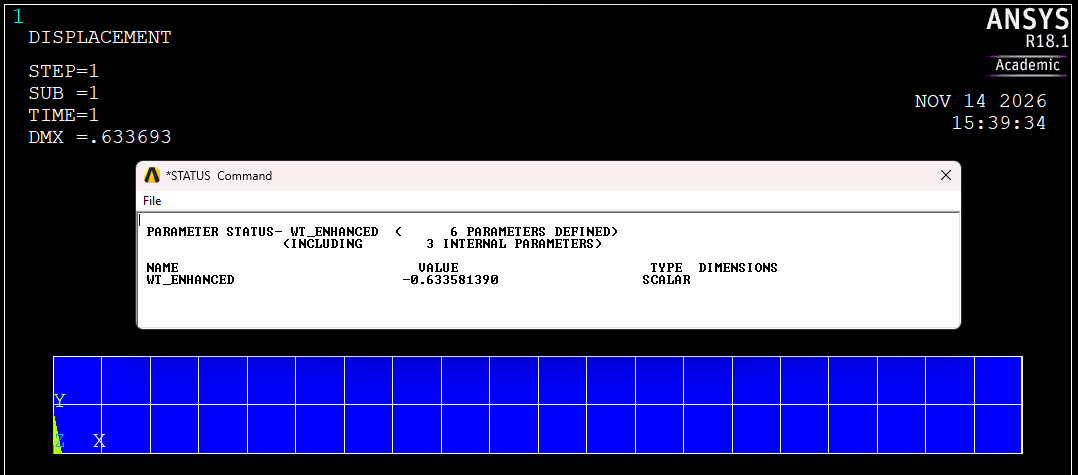
\includegraphics[width=0.72\linewidth]{figures/lab7_2_c_i.png}
\caption{Enhanced-strain SOLID185 result}
\label{lab7_enhanced}
\end{figure}

\begin{figure}[!h]
\centering
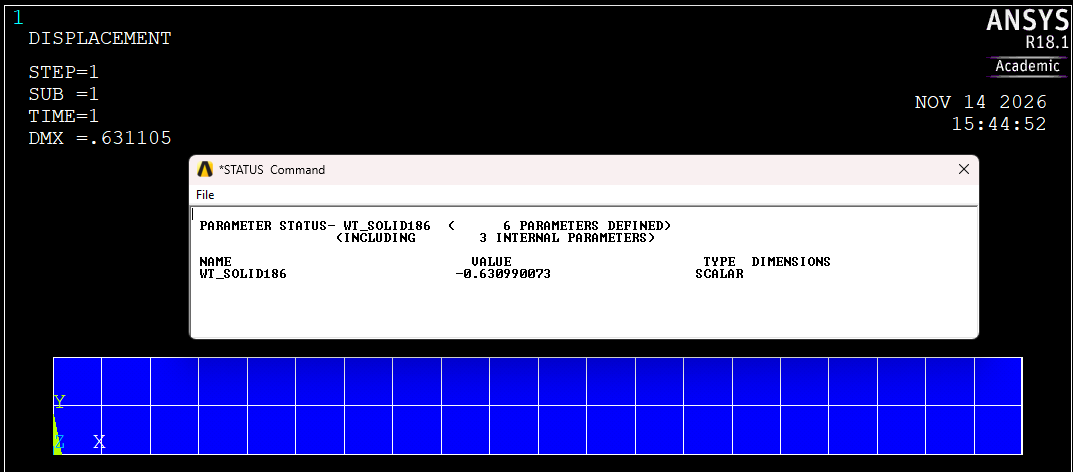
\includegraphics[width=0.72\linewidth]{figures/lab7_2_c_ii.png}
\caption{SOLID186 twenty-node brick result}
\label{lab7_solid186}
\end{figure}

\begin{figure}[!h]
\centering
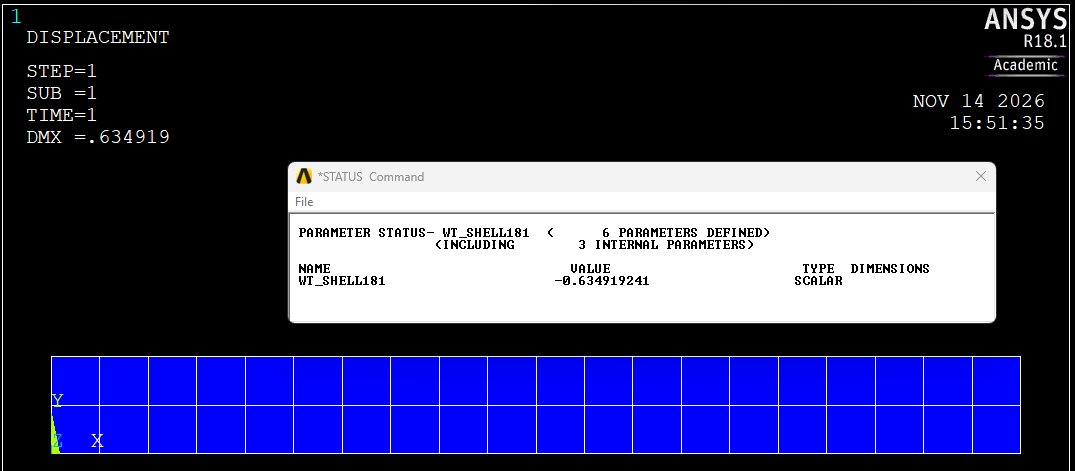
\includegraphics[width=0.72\linewidth]{figures/lab7_2_c_iii_corrected.png}
\caption{SHELL181 mid-surface result}
\label{lab7_shell}
\end{figure}

The sketch in Figure~\ref{lab7_element_sketch} illustrates the two mechanisms.
For a fully integrated eight-node brick, bending is approximated by linear
edge displacement. In a thin element under pure bending, the in-plane
displacements of the two transverse faces do not permit the element to
develop curvature without also acquiring a spurious transverse shear strain.
The element consequently stores artificial shear strain energy and appears
too stiff. This is shear locking.

With uniform reduced integration, only one point checks the element strain.
Some alternating nodal displacement patterns give zero strain at that point
even though the actual element is distorted. These are zero-energy
hourglass modes. Hourglass control supplies artificial stabilization, and
additional elements through the thickness provide more integration constraints.
The single-node load is useful only to reveal the mode; it is not a physical
load case for reporting the strip stiffness.

The enhanced-strain SOLID185, SOLID186, and SHELL181 formulations give nearly
the same tip displacement, within approximately \(0.6\%\). Their ratios
are close to unity and agree much better with the Euler--Bernoulli
reference than the locked full-integration SOLID185 result. The reduced-
integration model with four elements through the thickness also approaches
the beam reference, with a ratio of \(1.058\).

\subsection{Deformed Shapes and Stress Patterns}

The final displacement plot for the solid strip is shown in
Figure~\ref{lab7_solid_deformed}. The deformation is dominated by bending,
with zero displacement at the clamped end and maximum downward displacement
at the loaded end. The stress field changes sign through the thickness,
consistent with the bending relation
\[
\sigma_x(z)=\frac{M(x)z}{I},\qquad
M(x)=P(L-x).
\]
The stress is largest near the built-in end, where the bending moment is
maximum, and approaches zero towards the free end.

\begin{figure}[!h]
\centering
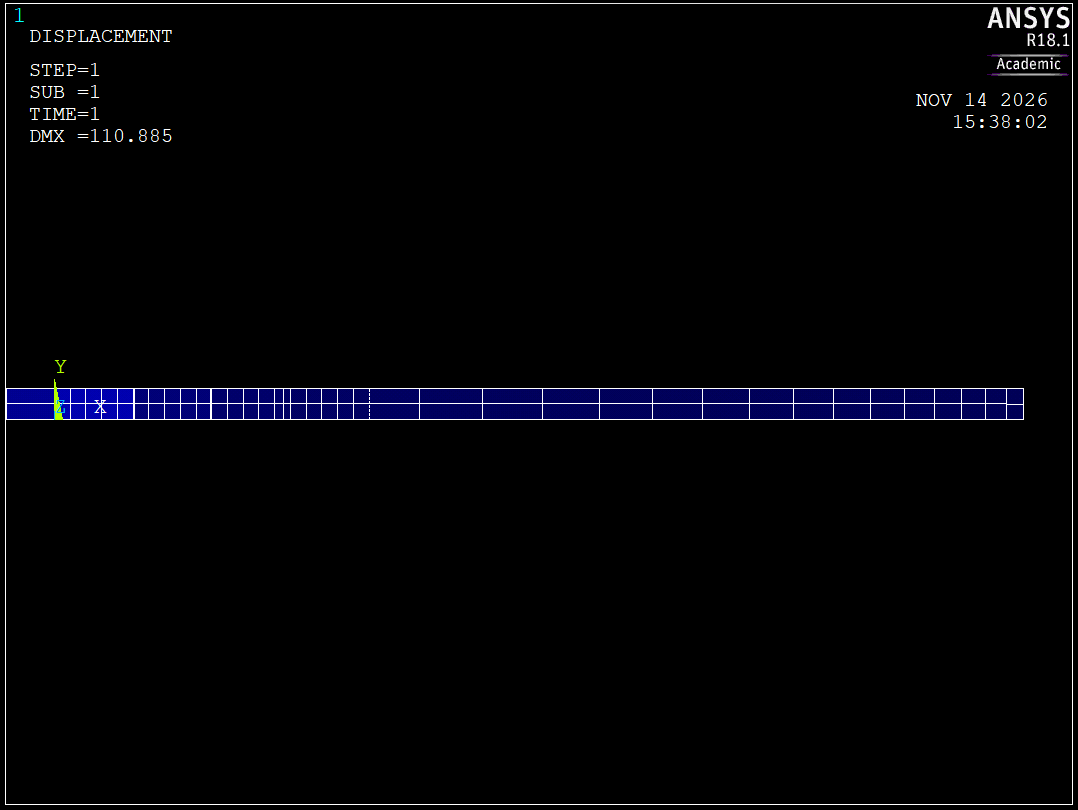
\includegraphics[width=0.72\linewidth]{figures/lab7_2_b_displacement_new.png}
\caption{Deformed solid-strip configuration}
\label{lab7_solid_deformed}
\end{figure}

\section{Discussion and Conclusion}

The square-plate study showed that the centre displacement converges rapidly
with mesh refinement. The \(8\times8\) and \(20\times20\) meshes produced
nearly identical centre deflections, so the finest mesh is adequate for the
reported stress and thickness studies. The top and bottom surface stresses
were equal in magnitude and opposite in sign, as required by bending
kinematics.

The thickness study demonstrated the limitation of thin-plate theory for
small \(a/t\). As the plate becomes thicker, transverse shear contributes a
larger fraction of the total displacement, and the Mindlin--Reissner
\texttt{SHELL181} result becomes larger than the Kirchhoff reference.

For the solid strip, full integration of the first-order
\texttt{SOLID185} element produced an overly stiff response because of shear
locking. Reduced integration alleviated the locking mechanism but exposed
hourglass behaviour under a single-node load. Enhanced strain and
\texttt{SOLID186} elements produced closely matching bending responses, while
\texttt{SHELL181} gave a similar result with substantially fewer through-
thickness degrees of freedom. The comparison confirms that element
formulation, mesh density, load distribution, and thickness modelling must
all be considered when evaluating a bending solution.